\title{CS 472 HW 5: Project 2}
\author{
        Aaron Havens\\
}
\date{\today}

\documentclass[12pt]{article}
\usepackage{amssymb} %maths
\usepackage{amsmath} %maths
\usepackage{graphicx}
\usepackage{array}
\graphicspath{{../figs/}}
\begin{document}
\maketitle\
\begin{center}
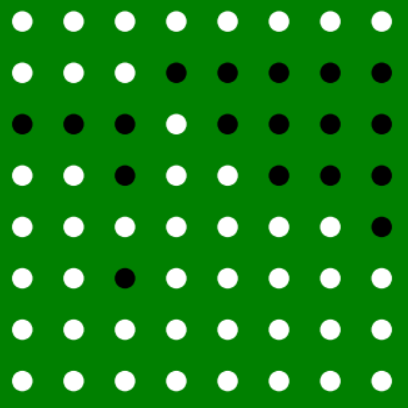
\includegraphics[scale=.8]{end_board}
\end{center}
\section{Othello $\alpha - \beta$ Depth Cut-off Observations}
\paragraph{Agent Strategy}The alpha beta playing agent designed operates on two basic scoring principles that govern its play space search. The first evaluation of a game state given a player is simply the difference in score between the player and the opponent. The 2nd component of the evaluation comes from a heavy weighting of the corner states, because they are seen as strategically valuable. This corner weighting appears to improve the game evaluation and agent will be compelled to select a move that leads to corner state over the depth horizon. 

\paragraph{Agent-Agent Performance} Based on these two scoring factors, the performance of an alpha-beta agent seems to be correlated to the depth-cutoff or look-ahead ability given to the agent. When playing to $\alpha-\beta$ agents against eachother with no corner weighting, the agent with the higher depth search will be more likely to win. Giving the agent the first move also seems to increase the likelihood of victory. When two agents are pit against eachother with same depth cut-off, but one agent is provided the corner score weighting evaluation function, that agent seems to be perform better most of the time. 

\paragraph{Efficiency and User experience} The run-time performance in relation to depth-cutoff is exponential and becomes very slow when the depth is greater than 5. Although it is feasible to plan to the end of the game for each agent move, it doesn't create a pleasant playing experience for the user on an average machine.
\end{document}